% Created by tikzDevice version 0.12.3.2 on 2022-02-17 22:23:42
% !TEX encoding = UTF-8 Unicode
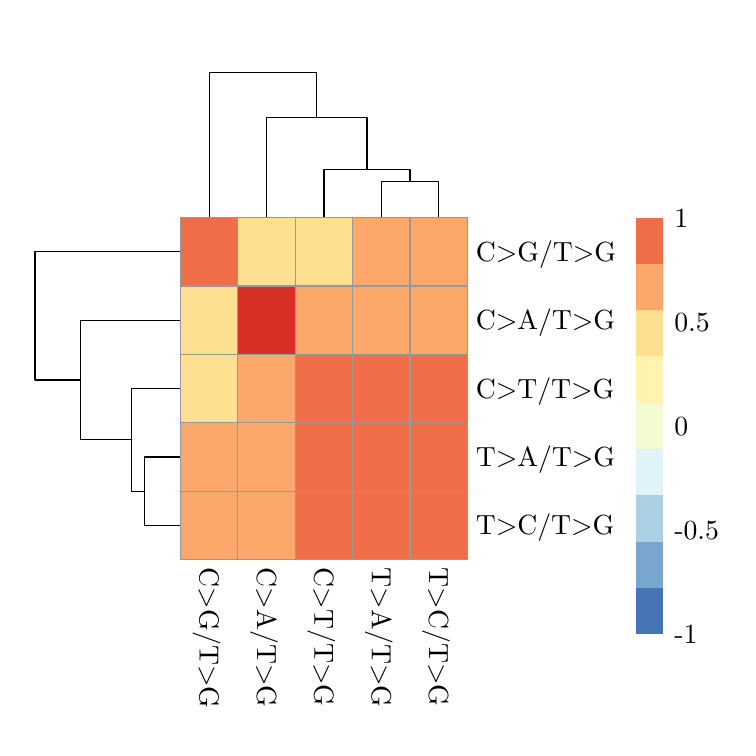
\begin{tikzpicture}[x=1pt,y=1pt]
\definecolor{fillColor}{RGB}{255,255,255}
\path[use as bounding box,fill=fillColor,fill opacity=0.00] (0,0) rectangle (252.94,252.94);
\begin{scope}
\path[clip] ( 55.21,184.31) rectangle (158.92,239.51);
\definecolor{drawColor}{RGB}{0,0,0}

\path[draw=drawColor,line width= 0.4pt,line join=round,line cap=round] (127.80,184.31) --
	(127.80,197.25) --
	(148.54,197.25) --
	(148.54,184.31);

\path[draw=drawColor,line width= 0.4pt,line join=round,line cap=round] (107.06,184.31) --
	(107.06,201.84) --
	(138.17,201.84) --
	(138.17,197.25);

\path[draw=drawColor,line width= 0.4pt,line join=round,line cap=round] ( 86.32,184.31) --
	( 86.32,220.39) --
	(122.62,220.39) --
	(122.62,201.84);

\path[draw=drawColor,line width= 0.4pt,line join=round,line cap=round] ( 65.58,184.31) --
	( 65.58,236.89) --
	(104.47,236.89) --
	(104.47,220.39);
\end{scope}
\begin{scope}
\path[clip] (  0.00, 60.72) rectangle ( 55.21,184.31);
\definecolor{drawColor}{RGB}{0,0,0}

\path[draw=drawColor,line width= 0.4pt,line join=round,line cap=round] ( 55.21, 97.80) --
	( 42.26, 97.80) --
	( 42.26, 73.08) --
	( 55.21, 73.08);

\path[draw=drawColor,line width= 0.4pt,line join=round,line cap=round] ( 55.21,122.52) --
	( 37.67,122.52) --
	( 37.67, 85.44) --
	( 42.26, 85.44);

\path[draw=drawColor,line width= 0.4pt,line join=round,line cap=round] ( 55.21,147.23) --
	( 19.13,147.23) --
	( 19.13,103.98) --
	( 37.67,103.98);

\path[draw=drawColor,line width= 0.4pt,line join=round,line cap=round] ( 55.21,171.95) --
	(  2.63,171.95) --
	(  2.63,125.61) --
	( 19.13,125.61);
\end{scope}
\begin{scope}
\path[clip] (  0.00,  0.00) rectangle (252.94,252.94);
\definecolor{drawColor}{gray}{0.60}
\definecolor{fillColor}{RGB}{239,110,72}

\path[draw=drawColor,line width= 0.4pt,line join=round,line cap=round,fill=fillColor] ( 55.21,159.59) rectangle ( 75.95,184.31);
\definecolor{fillColor}{RGB}{254,224,144}

\path[draw=drawColor,line width= 0.4pt,line join=round,line cap=round,fill=fillColor] ( 55.21,134.87) rectangle ( 75.95,159.59);

\path[draw=drawColor,line width= 0.4pt,line join=round,line cap=round,fill=fillColor] ( 55.21,110.16) rectangle ( 75.95,134.87);
\definecolor{fillColor}{RGB}{252,168,107}

\path[draw=drawColor,line width= 0.4pt,line join=round,line cap=round,fill=fillColor] ( 55.21, 85.44) rectangle ( 75.95,110.16);

\path[draw=drawColor,line width= 0.4pt,line join=round,line cap=round,fill=fillColor] ( 55.21, 60.72) rectangle ( 75.95, 85.44);
\definecolor{fillColor}{RGB}{254,224,144}

\path[draw=drawColor,line width= 0.4pt,line join=round,line cap=round,fill=fillColor] ( 75.95,159.59) rectangle ( 96.69,184.31);
\definecolor{fillColor}{RGB}{215,48,39}

\path[draw=drawColor,line width= 0.4pt,line join=round,line cap=round,fill=fillColor] ( 75.95,134.87) rectangle ( 96.69,159.59);
\definecolor{fillColor}{RGB}{252,168,107}

\path[draw=drawColor,line width= 0.4pt,line join=round,line cap=round,fill=fillColor] ( 75.95,110.16) rectangle ( 96.69,134.87);

\path[draw=drawColor,line width= 0.4pt,line join=round,line cap=round,fill=fillColor] ( 75.95, 85.44) rectangle ( 96.69,110.16);

\path[draw=drawColor,line width= 0.4pt,line join=round,line cap=round,fill=fillColor] ( 75.95, 60.72) rectangle ( 96.69, 85.44);
\definecolor{fillColor}{RGB}{254,224,144}

\path[draw=drawColor,line width= 0.4pt,line join=round,line cap=round,fill=fillColor] ( 96.69,159.59) rectangle (117.43,184.31);
\definecolor{fillColor}{RGB}{252,168,107}

\path[draw=drawColor,line width= 0.4pt,line join=round,line cap=round,fill=fillColor] ( 96.69,134.87) rectangle (117.43,159.59);
\definecolor{fillColor}{RGB}{239,110,72}

\path[draw=drawColor,line width= 0.4pt,line join=round,line cap=round,fill=fillColor] ( 96.69,110.16) rectangle (117.43,134.87);

\path[draw=drawColor,line width= 0.4pt,line join=round,line cap=round,fill=fillColor] ( 96.69, 85.44) rectangle (117.43,110.16);

\path[draw=drawColor,line width= 0.4pt,line join=round,line cap=round,fill=fillColor] ( 96.69, 60.72) rectangle (117.43, 85.44);
\definecolor{fillColor}{RGB}{252,168,107}

\path[draw=drawColor,line width= 0.4pt,line join=round,line cap=round,fill=fillColor] (117.43,159.59) rectangle (138.17,184.31);

\path[draw=drawColor,line width= 0.4pt,line join=round,line cap=round,fill=fillColor] (117.43,134.87) rectangle (138.17,159.59);
\definecolor{fillColor}{RGB}{239,110,72}

\path[draw=drawColor,line width= 0.4pt,line join=round,line cap=round,fill=fillColor] (117.43,110.16) rectangle (138.17,134.87);

\path[draw=drawColor,line width= 0.4pt,line join=round,line cap=round,fill=fillColor] (117.43, 85.44) rectangle (138.17,110.16);

\path[draw=drawColor,line width= 0.4pt,line join=round,line cap=round,fill=fillColor] (117.43, 60.72) rectangle (138.17, 85.44);
\definecolor{fillColor}{RGB}{252,168,107}

\path[draw=drawColor,line width= 0.4pt,line join=round,line cap=round,fill=fillColor] (138.17,159.59) rectangle (158.92,184.31);

\path[draw=drawColor,line width= 0.4pt,line join=round,line cap=round,fill=fillColor] (138.17,134.87) rectangle (158.92,159.59);
\definecolor{fillColor}{RGB}{239,110,72}

\path[draw=drawColor,line width= 0.4pt,line join=round,line cap=round,fill=fillColor] (138.17,110.16) rectangle (158.92,134.87);

\path[draw=drawColor,line width= 0.4pt,line join=round,line cap=round,fill=fillColor] (138.17, 85.44) rectangle (158.92,110.16);

\path[draw=drawColor,line width= 0.4pt,line join=round,line cap=round,fill=fillColor] (138.17, 60.72) rectangle (158.92, 85.44);
\end{scope}
\begin{scope}
\path[clip] (  0.00,  0.00) rectangle (252.94,252.94);
\definecolor{drawColor}{RGB}{0,0,0}

\node[text=drawColor,rotate=270.00,anchor=base west,inner sep=0pt, outer sep=0pt, scale=  1.00] at ( 62.13, 57.71) {C$>$G/T$>$G};

\node[text=drawColor,rotate=270.00,anchor=base west,inner sep=0pt, outer sep=0pt, scale=  1.00] at ( 82.88, 57.71) {C$>$A/T$>$G};

\node[text=drawColor,rotate=270.00,anchor=base west,inner sep=0pt, outer sep=0pt, scale=  1.00] at (103.62, 57.71) {C$>$T/T$>$G};

\node[text=drawColor,rotate=270.00,anchor=base west,inner sep=0pt, outer sep=0pt, scale=  1.00] at (124.36, 57.71) {T$>$A/T$>$G};

\node[text=drawColor,rotate=270.00,anchor=base west,inner sep=0pt, outer sep=0pt, scale=  1.00] at (145.10, 57.71) {T$>$C/T$>$G};
\end{scope}
\begin{scope}
\path[clip] (  0.00,  0.00) rectangle (252.94,252.94);
\definecolor{drawColor}{RGB}{0,0,0}

\node[text=drawColor,anchor=base west,inner sep=0pt, outer sep=0pt, scale=  1.00] at (161.93,168.51) {C$>$G/T$>$G};

\node[text=drawColor,anchor=base west,inner sep=0pt, outer sep=0pt, scale=  1.00] at (161.93,143.79) {C$>$A/T$>$G};

\node[text=drawColor,anchor=base west,inner sep=0pt, outer sep=0pt, scale=  1.00] at (161.93,119.07) {C$>$T/T$>$G};

\node[text=drawColor,anchor=base west,inner sep=0pt, outer sep=0pt, scale=  1.00] at (161.93, 94.36) {T$>$A/T$>$G};

\node[text=drawColor,anchor=base west,inner sep=0pt, outer sep=0pt, scale=  1.00] at (161.93, 69.64) {T$>$C/T$>$G};
\end{scope}
\begin{scope}
\path[clip] (  0.00,  0.00) rectangle (252.94,252.94);
\definecolor{fillColor}{RGB}{69,117,180}

\path[fill=fillColor] (219.64, 33.75) rectangle (229.68, 50.48);
\definecolor{fillColor}{RGB}{119,166,206}

\path[fill=fillColor] (219.64, 50.48) rectangle (229.68, 67.20);
\definecolor{fillColor}{RGB}{171,208,228}

\path[fill=fillColor] (219.64, 67.20) rectangle (229.68, 83.93);
\definecolor{fillColor}{RGB}{224,243,248}

\path[fill=fillColor] (219.64, 83.93) rectangle (229.68,100.66);
\definecolor{fillColor}{RGB}{244,251,210}

\path[fill=fillColor] (219.64,100.66) rectangle (229.68,117.39);
\definecolor{fillColor}{RGB}{254,244,175}

\path[fill=fillColor] (219.64,117.39) rectangle (229.68,134.12);
\definecolor{fillColor}{RGB}{254,224,144}

\path[fill=fillColor] (219.64,134.12) rectangle (229.68,150.85);
\definecolor{fillColor}{RGB}{252,168,107}

\path[fill=fillColor] (219.64,150.85) rectangle (229.68,167.58);
\definecolor{fillColor}{RGB}{239,110,72}

\path[fill=fillColor] (219.64,167.58) rectangle (229.68,184.31);
\definecolor{drawColor}{RGB}{0,0,0}

\node[text=drawColor,anchor=base west,inner sep=0pt, outer sep=0pt, scale=  1.00] at (233.69, 30.30) {-1};

\node[text=drawColor,anchor=base west,inner sep=0pt, outer sep=0pt, scale=  1.00] at (233.69, 67.94) {-0.5};

\node[text=drawColor,anchor=base west,inner sep=0pt, outer sep=0pt, scale=  1.00] at (233.69,105.58) {0};

\node[text=drawColor,anchor=base west,inner sep=0pt, outer sep=0pt, scale=  1.00] at (233.69,143.22) {0.5};

\node[text=drawColor,anchor=base west,inner sep=0pt, outer sep=0pt, scale=  1.00] at (233.69,180.87) {1};
\end{scope}
\end{tikzpicture}
